\documentclass[tikz,border=10pt]{standalone}
\usepackage[utf8]{inputenc}
\usepackage[T1]{fontenc}
\usepackage{lmodern}
\usetikzlibrary{arrows.meta,positioning,fit}
\definecolor{navy}{HTML}{15324B}
\definecolor{blue}{HTML}{2F80C1}
\definecolor{cyan}{HTML}{DCEFF7}
\definecolor{orange}{HTML}{E8873A}
\definecolor{green}{HTML}{3B8F72}
\tikzset{
  box/.style={draw=navy,rounded corners=3pt,very thick,align=center,
    minimum height=1.15cm,text width=3.0cm,fill=white,font=\sffamily\small},
  arr/.style={-{Latex[length=3mm]},very thick,navy},
  dep/.style={-{Latex[length=1mm,width=1.2mm]},semithick,navy},
  note/.style={font=\sffamily\small,align=center,text=navy}
}
\begin{document}
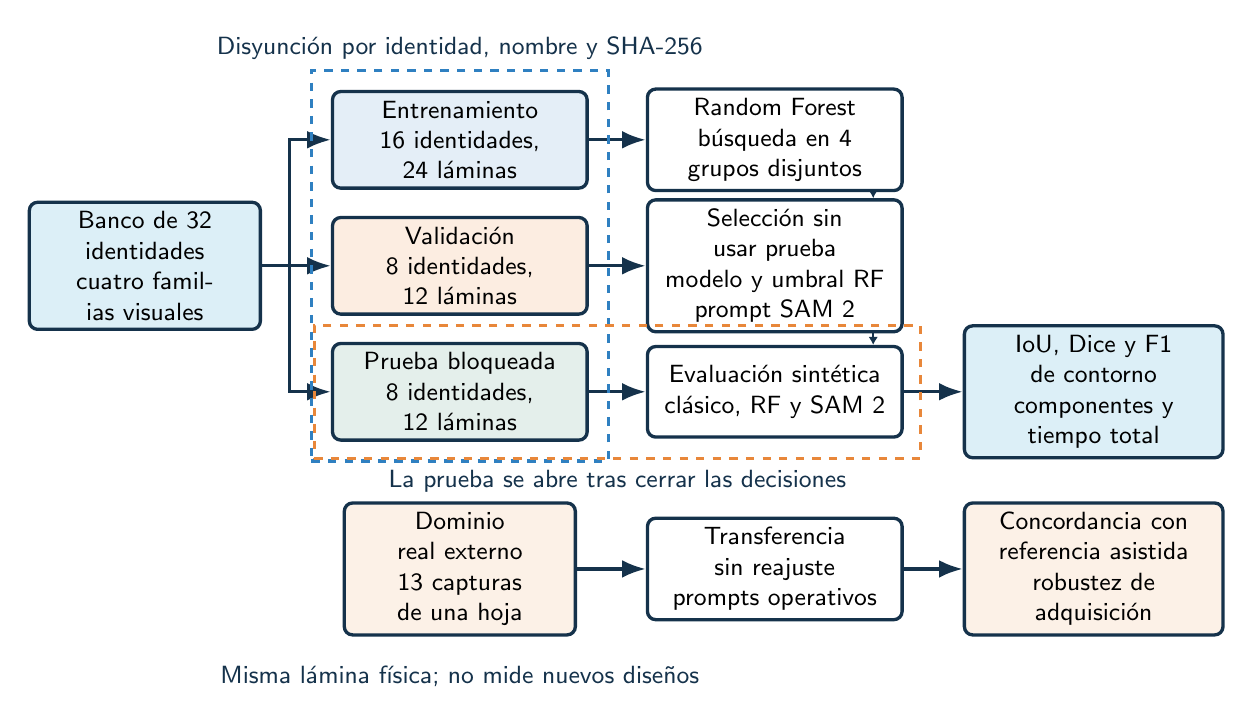
\begin{tikzpicture}[node distance=0.7cm and 0.85cm]
  \node[box,fill=cyan,text width=2.7cm] (bank) at (0,1.6)
    {Banco de 32\\identidades\\cuatro familias visuales};

  \node[box,fill=blue!13] (train) at (4.0,3.2)
    {Entrenamiento\\16 identidades, 24 láminas};
  \node[box,fill=orange!15] (validation) at (4.0,1.6)
    {Validación\\8 identidades, 12 láminas};
  \node[box,fill=green!14] (test) at (4.0,0.0)
    {Prueba bloqueada\\8 identidades, 12 láminas};
  \draw[arr] (bank.east) -- ++(0.35,0) |- (train.west);
  \draw[arr] (bank.east) -- (validation.west);
  \draw[arr] (bank.east) -- ++(0.35,0) |- (test.west);

  \node[box] (fit) at (8.0,3.2)
    {Random Forest\\búsqueda en 4 grupos disjuntos};
  \node[box] (select) at (8.0,1.6)
    {Selección sin usar prueba\\modelo y umbral RF\\prompt SAM 2};
  \node[box] (synthetic_eval) at (8.0,0.0)
    {Evaluación sintética\\clásico, RF y SAM 2};
  \draw[arr] (train)--(fit);
  \draw[arr] (validation)--(select);
  \draw[dep] ([xshift=1.25cm]fit.south)--([xshift=1.25cm]select.north);
  \draw[arr] (test)--(synthetic_eval);
  \draw[dep] ([xshift=1.25cm]select.south)--([xshift=1.25cm]synthetic_eval.north);

  \node[box,fill=cyan,text width=3.05cm] (synthetic_metrics) at (12.05,0.0)
    {IoU, Dice y F1 de contorno\\componentes y\\tiempo total};
  \draw[arr] (synthetic_eval)--(synthetic_metrics);

  \node[box,fill=orange!12,text width=2.7cm] (real) at (4.0,-2.25)
    {Dominio real externo\\13 capturas de una hoja};
  \node[box] (real_eval) at (8.0,-2.25)
    {Transferencia sin reajuste\\prompts operativos};
  \node[box,fill=orange!12,text width=3.05cm] (real_metrics) at (12.05,-2.25)
    {Concordancia con referencia asistida\\robustez de adquisición};
  \draw[arr] (real)--(real_eval);
  \draw[arr] (real_eval)--(real_metrics);

  \node[draw=blue,dashed,very thick,fit=(train)(validation)(test),inner sep=7pt,
    label={[note]above:Disyunción por identidad, nombre y SHA-256}] {};
  \node[draw=orange,dashed,very thick,fit=(test)(synthetic_eval),inner sep=6pt,
    label={[note]below:La prueba se abre tras cerrar las decisiones}] {};
  \node[note,below=0.25cm of real]
    {Misma lámina física; no mide nuevos diseños};
\end{tikzpicture}
\end{document}
